% !TEX encoding = UTF-8 Unicode

\chapter{HTML5-Anwendungsentwicklung}

Wird eine Anwendung mit HTML5 entwickelt, so wird eine Kombination der drei Technologien HTML, CSS und JavaScript verwendet. Jede dieser Technologien deckt einen gewissen Aspekt der HTML5-Anwendungsentwicklung ab. HTML wird verwendet um Inhalte festzulegen, mit CSS wird das Layout festgelegt und JavaScript bestimmt das Verhalten. Soweit möglich sollte diese Trennung auch eingehalten werden. Da Inhalt und Layout aber auch dynamisch angepasst werden, greift JavaScript auch in diese Bereiche ein.

\section*{Dynamische Anpassung der Benutzeroberfläche}

Wenn im Bezug auf die vorliegende HTML5-Anwendung von Inhalt gesprochen wird, so sind damit die Steuerelemente selbst sowie ihre Gruppierung gemeint. Das Layout bestimmt die Anordnung der Steuerelemente und welche Steuerelemente angezeigt werden. Im vorherigen Abschnitt ist angesprochen worden, dass sich die Anzahl der angezeigten Steuerelemente sowie ihr Layout je nach Fenstergröße ändert. Diese Änderung wird mittels JavaScript durchgeführt. Die Bibliothek jQuery \autocite{jquery} bietet eine Funktion, mit welcher sich einzelne oder mehrere HTML-Elemente über CSS-Selektoren auswählen lassen. Die HTML-Attribute und CSS-Eigenschaften der selektierten Elemente können dann manipuliert werden. Die jQuery-Funktion wird entweder mit \verb+jQuery+ oder dem Dollar-Zeichen aufgerufen.

\begin{figure}[htbp]
	\centering
	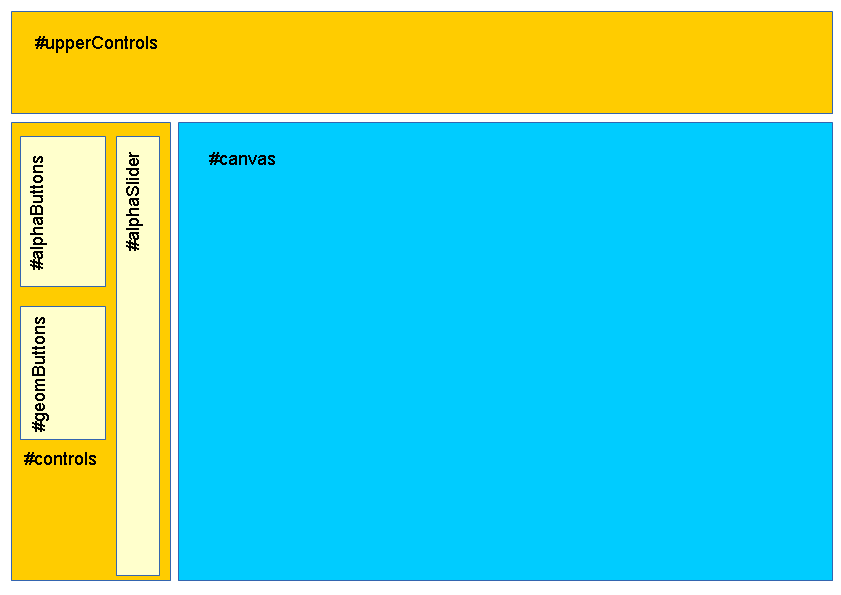
\includegraphics[scale=0.9]{../bilder/layout.png}
	\caption{Layout der $\alpha$-Shapes HTML5-Applikation}
	\label{fig:layout}
\end{figure}

In Abbildung~\ref{fig:layout} ist das Layout der Applikation dargestellt. Die Bezeichner mit einer vorangestellten Raute beziehen sich auf IDs von HTML-Elementen. Die Raute wird CSS-Selektoren vorangestellt, welche ein Element nach ihrer ID auswählen. Die in Gelbtönen eingefärbten Blöcke stellen Div-Elemente dar. Der blaue Block ist das Canvas-Element, auf welchem die Punktmenge und alle anderen Diagramme gezeichnet werden. In \verb+alphaButtons+ sind alle Buttons enthalten, welche die Darstellung von $\alpha$-Shape, -Hülle und -Kreisscheiben steuern. In \verb+geomButtons+ sind alle Buttons enthalten, welche die Darstellung von Delaunay-Graphen und Voronoi-Diagrammen steuern.

Das nun gezeigte Codebeispiel befindet sich in dem Resize-Event-Handler des Window-Elements. In Listing~\ref{upperSideControls} wird demonstriert, wie zwischen Darstellung im Hoch- und Querformat bzw. zwischen seitlichen und oberen Steuerelementen umgeschaltet wird. Hierzu sei angemerkt, dass alle Buttons in \verb+geomButtons+ zu einer Klasse \verb+geomButton+ gehören. CSS-Selektoren, welche sich auf eine Klasse beziehen, wird ein Punkt vorangestellt.

\begin{lstlisting}[float = htbp, caption={Umstellen zwischen Hoch- und Querformat},label=upperSideControls]
if (window.innerHeight > window.innerWidth) {
	$('.geomButton').prop('checked', false);
	$('.geomButton').button('refresh');
	$('#upperControls').css('display', '');
	$('#controls').css('display', 'none');
} else {
	$('#upperControls').css('display', 'none');
	$('#controls').css('display', '');        
}
\end{lstlisting}

Die jQuery-Funktion liefert ein jQuery-Objekt zurück. Mit den Methoden \verb+prop+ und \verb+css+ können HTML-Attribute bzw. CSS-Eigenschaften von den durch das jQuery-Objekt selektierten Elementen verändert werden. Die Methode \verb+button+ wird durch die Bibliothek jQueryUI hinzugefügt. Die verwendeten Button-Steuer\-elemente sind eigentlich HTML-Checkbox-Elemente. Mit jQueryUI können diese als Toggle-Buttons dargestellt werden, welche durch ihre Größe besser mit dem Finger zu bedienen sind. Da in der Darstellung im Hochformat die Buttons für Delaunay-Graphen sowie Voronoi-Diagramme nicht sichtbar sind, wird die Darstellung dieser Diagramme deaktiviert.

\section*{Event-Handler für Touch- und Mausbedienung}

Da mobile Geräte über Touchdisplays bedient werden, müssen die entsprechenden Event-Handler implementiert werden.

\begin{lstlisting}[float = htbp, caption={Zuweisen der Event-Handler an das Canvas-Element},label=canvasEvents]
$('#canvas').mousedown(CanvasController.handleDragStart);
$('#canvas').mousemove(CanvasController.handleDragMove);
$('#canvas').mouseup(CanvasController.handleDragEnd);

$('#canvas').bind('touchstart',
	CanvasController.handleTouchDragStart);
$('#canvas').bind('touchmove',
	CanvasController.handleTouchDragMove);
$('#canvas').bind('touchend',
	CanvasController.handleTouchDragEnd);
\end{lstlisting}

Listing~\ref{canvasEvents} zeigt die Zuweisung der Event-Handler für Mouse- und Touch-Ereignisse. Die Implementierung dieser Event-Handler-Funktionen ist aber fast identisch. Sie unterscheiden sich nur in der Ermittlung der Position des Ereignisses und ob an dieser Position schon ein Punkt existiert. Für Touchbedienung müssen ggf. mehrere Touch-Ereignisse (für mehrere Finger) ausgewertet werden und Punkte in einem größeren Umkreis um die Position des Events berücksichtigt werden.

\begin{lstlisting}[float = htbp, caption={Touch-Event-Handler},label=touchEvent]
var x = event.originalEvent.targetTouches[0].pageX -
	$('#canvas').offset().left;
var y = event.originalEvent.targetTouches[0].pageY -
	$('#canvas').offset().top;
var pointIndex = Misc.getIndexOfElementWithMinimalDistance(
	UserData.points, new Vector(x, y), Vector.calcDist,
	CanvasController.maxPointDistTouch);
\end{lstlisting}

Listing~\ref{touchEvent} zeigt die Ermittlung der Koordinaten eines Touch-Events sowie die Ermittlung des Index des Punkts in einem Array, welcher am nächsten zu den Koordinaten des Ereignisses liegt. Falls der Abstand des nächsten Punktes einen Maximalwert überschreitet oder das Array leer ist, wird der Wert $-1$ zurückgegeben. \verb+UserData.points+ ist das Array mit den Vektoren der Punkte, welche auf der Zeichenfläche dargestellt werden. Mit \verb+new Vector(x, y)+ wird ein Vektor mit den Koordinaten des Events zum Vergleich mit den Array-Elementen erzeugt. \verb+Vector.calcDist+ ist eine Funktion, welche die Distanz zwischen Vektoren berechnet. Die Konstante \verb+CanvasController.maxPointDistTouch+ legt den Radius des Umkreises fest, in welchem ein Punkt mittels einer Berührung selektiert werden kann. 

\section*{JavaScript und Klassen}
In der Entwicklung objektorientierter Software wird Code üblicherweise in Klassen organisiert. JavaScript bietet dieses Konstrukt nicht an. Allerdings lassen sich durch JavaScript-Spracheigenschaften Klassen nachbilden. Dies wird z.B. in \autocite{Flanagan2011} beschrieben. Listing~\ref{vectorClass} zeigt eine Klasse \verb+Vector+ mit den Attributen \verb+x+ und \verb+y+, einer Methode \verb+add+ und einer statischen Methode \verb+calcDist+.

\begin{lstlisting}[float = htbp, caption={Eine Vektor-Klasse},label=vectorClass]
function Vector(x, y) {
    this.x = x;
    this.y = y;    
};

Vector.prototype = {
    constructor: Vector,
    add : function(v) {
        return new Vector(this.x + v.x, this.y + v.y);
    }, ...
};

Vector.calcDist = function(v1, v2) {
    var dist = v1.sub(v2).abs();
    return dist;
};
\end{lstlisting}

Die Funktion \verb+Vector+ wird Konstruktor genannt. In ihr werden die Attribute festgelegt. Im Prototypen werden die Methoden definiert. Statische Methoden werden dem Konstruktor als Eigenschaft hinzugefügt.

Zudem lassen sich in Klassen auch zusätzliche Einschränkungen wie Sichtbarkeit und Veränderbarkeit von Objekt- und Klasseneigenschaften definieren. JavaScript bietet diese Möglichkeiten nicht. Sichtbarkeit und Veränderbarkeit können durch jsDoc-Kommentare, wie in \autocite{useJsDoc} beschrieben, festgelegt werden. jsDoc wird ähnlich wie JavaDoc verwendet. Ein Compiler, wie z.B. der hier verwendete Closure-Compiler von Google \autocite{closureTools}, kann die Einhaltung von Sichtbarkeit und Veränderbarkeit überprüfen, sie kann aber nicht durch den Interpreter erzwungen werden. Listing~\ref{vectorClassImmutable} zeigt wie die Attribute der Klasse \verb+Vector+ zu Konstanten gemacht werden können.

\begin{lstlisting}[float = htbp, caption={Eine Vektor-Klasse mit konstanten Attributen},label=vectorClassImmutable]
function Vector(x, y) {
    /**
     * @const
     */
    this.x = x;
    /**
     * @const
     */
    this.y = y;    
};
\end{lstlisting}

\section*{JavaScript und Typsicherheit}

JavaScript ist eine dynamisch typisierte Sprache, welche Duck-Typing benutzt. Das bedeutet, es können zur Laufzeit Eigenschaften zu Objekten hinzugefügt werden und der Interpreter prüft erst zur Laufzeit, ob ein Objekt eine benötigte Eigenschaft besitzt. Ist eine benötigte Eigenschaft nicht vorhanden, so kommt es zu einem Laufzeitfehler.

Mit Hilfe der vorher schon benutzten jsDoc-Kommentare können Typinformationen zu Variablen hinzugefügt werden. Ein Compiler kann dann überprüfen, ob den so deklarierten Variablen auch Objekte des richtigen Typs zugewiesen werden und ob das Objekt über die benötigten Eigenschaften verfügt. Listing~\ref{vectorClassTypes} zeigt wie der Klasse \verb+Vector+ Typinformationen hinzugefügt werden können.

\begin{lstlisting}[float = htbp, caption={Eine Vektor-Klasse mit Typinformationen},label=vectorClassTypes]
/**
 * Represents a 2D vector.
 * 
 * @constructor
 * @param {number} x coordinate
 * @param {number} y coordinate
 */
function Vector(x, y) {
    /**
     * @const
     * @type number
     */
    this.x = x;
    /**
     * @const
     * @type number
     */
    this.y = y;    
};
...
    /**
     * Vector addition
     * 
     * @param {Vector} v 2nd summand
     * @returns {Vector} sum of this vector and v
     */
    add : function(v) {
        return new Vector(this.x + v.x, this.y + v.y);
    },
...
\end{lstlisting}

Zusätzlich zu den Typinformationen wurden der Konstruktor- und die Methoden-Köpfe auch noch kommentiert. Das jsDoc-Projekt stellt ein Tool \autocite{jsDoc} zur Verfügung, mit welchem aus dem kommentierten Quellcode eine API-Dokumentation im HTML-Format erstellt werden kann.

\section*{JavaScript Unit-Tests} 

Eine andere Möglichkeit vor der Ausführung des Programms Fehler zu erkennen sind Unit-Tests. Die Bibliothek Jasmine \autocite{jasmine} ermöglicht das Erstellen und Ausführen von Unit-Tests. Listing~\ref{vectorClassUnitTest} zeigt einen Unit-Test zur \verb+add+-Methode der \verb+Vector+-Klasse.

\begin{lstlisting}[float = htbp, caption={Ein Unit-Test zur Vektoraddition},label=vectorClassUnitTest]
describe('Vector', function() {
    it('adds vectors', function() {
        var vector1 = new Vector(5,7);
        var vector2 = new Vector(1,2);
        var expected = new Vector(6,9);
        var result = vector1.add(vector2);
        
        expect(expected.equals(result)).toBe(true);
    });
});
\end{lstlisting}


\section*{JavaScript Vererbung}

In der Entwicklung objektorientierter Software wird üblicherweise zwischen der Implementierungs- und der Schnittstellenvererbung unterschieden. JavaScript unterstützt das Konzept der Prototypen-basierten Vererbung. Damit können Implementierungen vererbt werden. Dies wird auch in \autocite{Flanagan2011} beschrieben. 


\begin{lstlisting}[float = htbp, caption={Eine AVL-Baum-Klasse},label=treeClass]
/**
 * @constructor
 */
function Tree() {
...
};
Tree.prototype = {
	constructor: tree;
	...
};

/**
 * @constructor
 * @extends Tree
 */
function FortuneTree() {
...
};

FortuneTree.prototype = Object.create(Tree.prototype);
FortuneTree.prototype.constructor = FortuneTree;

FortuneTree.prototype.insertNewArcNode =
	function(eventLocation, edgeList) {
...
}
\end{lstlisting}

Listing~\ref{treeClass} zeigt eine Klasse \verb+Tree+, von welcher eine Klasse \verb+FortuneTree+ abgeleitet ist. Bei \verb+Tree+ handelt es sich um einen AVL-Baum. In Fortunes Algorithmus werden innere Knoten und Blätter unterschieden. Das Einfügen eines Knotens in den AVL-Baum in Fortunes Algorithmus umfasst einige sehr spezielle Schritte. Darum ist das einfügen eines Knotens in der speziellen \verb+FortuneTree+-Klasse implementiert.

\chapter{Projektstruktur}

Alle der im vorhergehenden Kapitel beschriebenen Hilfsmittel bei der Entwicklung mit HTML5 bzw. JavaScript finden sich in der Projektstruktur wieder. Das HTML5-Anwendungsprojekt ist im Repository \verb+AlphaShapeSeidinger+ unter \verb+projekte/alpha_shapes_html5+ zu finden. Der wichtigste Ordner unterhalb dieses Ordners ist der Ordner \verb+public_html+. In ihm befinden sich alle HTML-, CSS- und JavaScript-Dateien. Hier wird kurz der Inhalt von \verb+public_html+ beschrieben:

\begin{itemize}
\item \verb+index.html+: Einbindung der CSS-Stylesheets und aller JavaScript-Dateien, Definition aller Steuerelement sowie deren Gruppierung
\item \verb+css/custom-ui.css+: Definition aller statischen Layout-Aspekte
\item \verb+data/simple_point_set.json+: Initiale Punkt\-menge im JSON-For\-mat
\item \verb+js/libs+: Alle eingesetzten JavaScript-Bibliotheken
\item \verb+js/geom+: Geometrische Datentypen
\item \verb+js/ds+: Datenstrukturen
\item \verb+js/algo+: Algorithmen
\item \verb+js/util+: Hilfsfunktionen
\item \verb+js/ui+: Event-Handler
\item \verb+js/compiled+: Compiler-generierter JavaScript-Code
\item \verb+js/README.md+: Quelle für Index-Seite der jsDoc-API-Dokumentation
\item \verb+test+: Jasmine Bibliothek sowie Unit-Tests
\item \verb+test/SpecRunner+: HTML-Datei zum Ausführen der Unit-Tests
\end{itemize}

Die vorher beschriebenen Werkzeuge befinden sich im Ordner des Anwendungsprojekts unterhalb des Ordners \verb+tools+:

\begin{itemize}
\item \verb+closure/compiler.jar+: Closure-Compiler
\item \verb+jsdoc/jsdoc+: Tool zur Erstellung von jsDoc-API-Dokumentation
\item \verb+check.bat+: Führt den Closure-Compiler mit einem hohen Warning-Level aus.
\item \verb+compile.bat+: Führt den Closure-Compiler mit den Standard-Einstellungen aus und legt das Ergebnis in das JavaScript-Quellcode-Verzeichnis.
\item \verb+doc.bat+: Führt das jsDoc-Tool aus und legt die API-Dokumentation in das Verzeichnis \verb+public_html/api+. Dieses Verzeichnis wird von Subversion ignoriert.
\end{itemize}
